\documentclass[twoside,11pt]{article}

% Any additional packages needed should be included after jmlr2e.
% Note that jmlr2e.sty includes epsfig, amssymb, natbib and graphicx,
% and defines many common macros, such as 'proof' and 'example'.
%
% It also sets the bibliographystyle to plainnat; for more information on
% natbib citation styles, see the natbib documentation, a copy of which
% is archived at http://www.jmlr.org/format/natbib.pdf

% Available options for package jmlr2e are:
%
%   - abbrvbib : use abbrvnat for the bibliography style
%   - nohyperref : do not load the hyperref package
%   - preprint : remove JMLR specific information from the template,
%         useful for example for posting to preprint servers.
%
% Example of using the package with custom options:
%
% \usepackage[abbrvbib]{jmlr2e}

\usepackage{jmlr2e}

% Definitions of handy macros can go here

\newcommand{\dataset}{{\cal D}}
\newcommand{\fracpartial}[2]{
    \frac{\partial #1}{\partial  #2}
}

% Heading arguments are {volume}{year}{pages}{date submitted}{date published}{paper id}{author-full-names}

\jmlrheading{1}{2000}{1-48}{4/00}{10/00}{meila00a}{Marina Meil\u{a} and Michael I. Jordan}

% Short headings should be running head and authors last names

\ShortHeadings{jax-unirep: A user-centered, performant reimplentation of UniRep in JAX}{Kummer, Jayapurna and Ma}
\firstpageno{1}

\begin{document}

\title{jax-unirep: Accelerated and User-Friendly Protein Machine Learning with JAX}

\author{
    \name Arkadij Kummer \email arkadij.kummer@novartis.com \\
    \addr Global Discovery Chemistry\\
    Novartis Institutes for Biomedical Research\\
    Basel, Switzerland
    \AND
    \name Ivan Jayapurna \email ivanfj@berkeley.edu \\
    \addr University of California\\
    Berkeley, CA, USA
    \AND
    \name Eric J. Ma \email eric.ma@novartis.com \\
    \addr NIBR Informatics\\
    Novartis Institutes for Biomedical Research\\
    Cambridge, MA, USA
}

\editor{}

\maketitle

\begin{abstract}%   <- trailing '%' for backward compatibility of .sty file
We provide a significantly upgraded version of UniRep, jax-unirep,
a recurrent neural network model trained on 24 million protein sequences,
with significant speed improvements,
API enhancements,
and reliability upgrades.
jax-unirep is implemented in JAX,
and takes advantage of JAX's programming model
to provide up to 100X speedup over the original implementation.
Surrounding the package are API enhancements
that support the "machine learning in protein engineering" workflow,
including proposing new sequences to sample,
writing end-to-end differentiable models that involve UniRep as a component,
and weight tuning,
all of which require minimal user intervention.
\verb|jax-unirep| has easily accessible documentation,
extensive (96\%) code test coverage,
automatic testing and docs redeployment,
readily copy-pasteable examples for workflow pieces,
and has enjoyed growing community adoption.
\end{abstract}

\begin{keywords}
  Recurrent Neural Networks, Machine Learning Application, Protein Engineering
\end{keywords}

\section{Introduction}

UniRep is a recurrent neural network,
trained using self-supervision
on 24 million protein sequences
to predict the next amino acid in a sequence (\cite{alley2019unified}).
Its most powerful model allows for embedding
arbitrary length sequences in a 1900-long feature vector
that can be used as the input to a downstream model
for unsupervised clustering or supervised prediction of protein properties.

The original model (also referred to here as \verb|tf-unirep|)
was implemented in TensorFlow 1.13 (\cite{abadi2016tensorflow}).
While test-driving \verb|tf-unirep|, we observed two issues
that hindered us from using it productively.
The first is that the original implementation
took an abnormally long amount of time to process multiple sequences,
requiring on the order of dozens of seconds to process tens of sequences.
The second was that its API was unwieldy,
and could have been simplified for protein engineers
who might not necessarily be programming-savvy.

In the presented library, we present a significant set of upgrades
over the original implementation.
Firstly, we accelerated the model 100X over the original,
and provide a benchmark comparison on the most common use case for UniRep.
Secondly, we added a library of APIs
that ease the usage of the model in protein engineering workflows,
as well as neural network layer definitions
that allow its inclusion in end-to-end differentiable models.
Thirdly, we provide extensive software testing,
much beyond what was provided in the original,
to facilitate further development work
and build user confidence in the package.
Finally, we provide documentation for the model,
including introductory and advanced workflows,
and contribution instructions.

\section{Architecture and Design}

\subsection{Top-level API}

\verb|jax-unirep|'s top-level API provides direct access
to user-facing functions:
(1) \verb|get_reps| for a continuous, 1900-long vector representation of a protein sequence,
(2) \verb|fit| and \verb|evotune| for "one-touch" evolutionary tuning of the model,
and
(3) \verb|sample_one_chain| to perform \textit{in silico} scoring of newly suggested mutants.
These cover the majority of tasks in a computational protein engineer's workflow
that will also involve a machine learning model for scoring of mutants.

\subsection{Model Implementation}

We treat the core model implementation as a function
that accepts a dictionary of parameters and input data.
That core function is in a sufficiently generic form (Python function)
that it can be easily incorporated into neural network layers.
As a demonstration, we wrote \verb|stax|-compatible layers,
though in principle the layers can be made Keras- or PyTorch-compatible easily,
thanks to the core functions being written in generic Python and NumPy.
Because neural network layers are nothing more than math functions
composed into higher-order functions,
we believe this architecture facilitates maximal portability
across deep learning APIs.

\subsection{Acceleration with JAX}

\begin{figure}[!tpb]
    \centerline{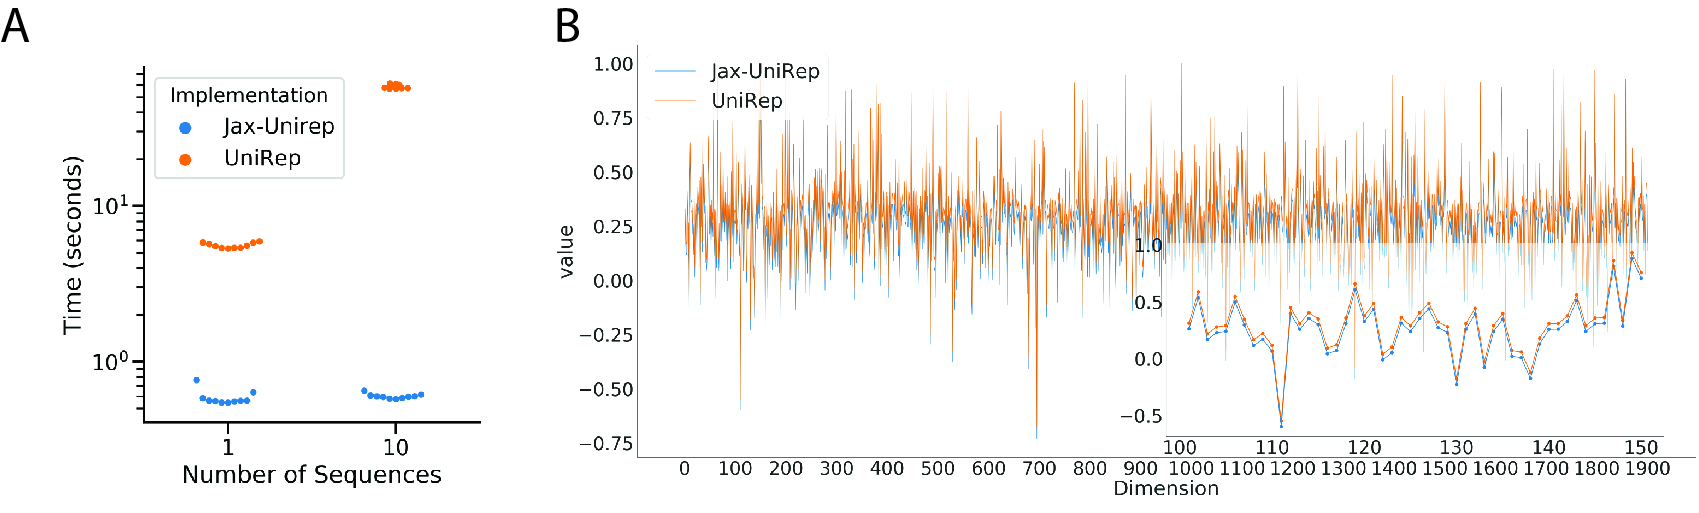
\includegraphics[width=6in]{fig01.jpg}}
    \caption{
        A. Speed comparison between the original implementation (UniRep)
        and our re-implementation (jax-unirep).
        Both one and ten random sequences of length ten
        were transformed by both implementations.
        B. Comparison of the average hidden state between the implementations
        when transforming the same sequence.
        The inset shows a slice of length 50 out of the total 1900 dimensions.
    }
    \label{fig:fig01}
\end{figure}

To investigate the performance of \verb|tf-unirep|,
we used Python's \verb|cProfile| facility to identify speed bottlenecks.
On the basis of this, we hypothesized that the cause of speed problems
was graph compilation in TF1.x,
and that we could obtain speedups by using
a non-graph-compiled tensor library.

There were three options available: TF2.x, PyTorch (\cite{pytorch})
and JAX (\cite{jax2018github}).
We chose JAX, because it provides automatic differentiation
on top of the idiomatic NumPy API (\cite{oliphant2006guide}),
In our reimplementation of the model,
we took advantage of JAX's \verb|lax.scan| function,
which allowed us to write performant RNN loops.
We also used \verb|vmap| for performant mapping of a function
over leading tensor axes
and \verb|jit| to leverage just-in-time compilation.
Together, we achieved at least two order of magnitudes speed-up
over the original implementation.

\section{Significant Software Improvements}

\subsection{Speed enhancements}

In a formal speed comparison, we found that \verb|jax-unirep|
performed up to 100X faster on the task of computing protein representations
(using the \verb|get_reps()| function) (Figure 1A\vphantom{\ref{fig:fig01}}).
We did not test more than 10 sequences
as the original unirep implementation would have taken
an unreasonably long amount of time to run
when using the comparable \verb|babbler.get_reps()| class method.
Speed comparisons were performed on a single core of a 24-core
CentOS7 workstation running Intel Xeon processors at 3.6 GHz
with at least 7 replicates.

\subsection{Batched processing of protein features}

Batching multiple sequences is one place where \verb|jax-unirep|
is significantly more user-friendly than \verb|tf-unirep|.
In \verb|tf-unirep|, to process multiple sequences,
an end-user would call \verb|babbler.get_reps(sequence)| in a loop,
essentially repeatedly paying the TensorFlow graph compilation penalty.
Alternatively, users would have to manually preprocess sequences
into the tensorized embedding using custom code
before passing them into the UniRep model.
This extra preprocessing step introduces room for user error,
impeding reproducibility of model usage results.

With \verb|jax-unirep|,
to obtain numeric representations of single and multiple protein sequences,
end-users use the high-level function \verb|get_reps()|,
which we have designed to accept single sequences and multiple sequences.
Sequences need not necessarily be of the same length.
Internally, conversion from strings to tensors happens automatically,
eliminating one source of user error affecting modelling results,
thereby guaranteeing consistency between model usage runs.

\subsection{Evolutionary tuning}

"Evotuning" is fine-tuning of the UniRep weights
for a defined collection
of evolutionarily-related protein sequences (\cite{alley2019unified})
that the end-user has curated.
Here, we provide a \verb|fit()| function to perform this task,
in which most of the code necessary for preprocessing the sequences
and performing gradient updates to the weights
are abstracted away from the end-user.
Additionally, automatic checkpointing
into a user-specified directory is available,
allowing users to select
which "evotuned" weights along the optimization path
they wish to use.

\subsection{Software testing and documentation}

We also provide software tests and documentation,
two pieces that were lacking in the original \verb|tf-unirep|.
In particular, our test suite covers over 96\% of the codebase;
in contrast to the original, which had no testing.
Additionally, documentation is provided on advanced workflow pieces
that can be \textit{modularly} incorporated
into a computational protein engineer's workflow,
with reference code in the docs provided.
Finally, we welcome community contributions.
To facilitate this process,
documentation is provided to help newcomer contributors.

\section{Reimplementation Verification}

To check that \verb|jax-unirep| was implemented correctly,
we computed numeric representations for single protein sequences
using the original and the reimplementation.
Figure 1B\vphantom{\ref{fig:fig01}} shows, for one example sequence,
that the representations are identical;
the difference in the traces were injected after computation
merely to visually separate them.

\section{Discussion and Future Work}

Through our reimplementation of UniRep,
we have effectively provided it with non-trivial upgrades
over the original.
Having verified its correctness in reimplementation,
we have improved the API, added software tests,
and sped up model forward pass speed by nearly 100X,
all of which are significant upgrades over the original implementation.
Because of the API efforts,
users have commented on our issue tracker and in pull requests
that it is a joy and delight to use,
and it is being incorporated into the \verb|bio-embeddings| package.

Significant effort was invested in accelerating, refactoring, documenting,
and testing the \verb|babbler1900| model.
This was the model with the largest "capacity" by number of parameters),
and is the most powerful of the three described in the original manuscript.
Future work includes implementing
the \verb|babbler256| and \verb|babbler64| models,
as well as continuing to serve the protein machine learning community
with workflow-oriented APIs.

\acks{We would like to acknowledge the original UniRep authors
for open sourcing their implementation,
our colleagues at NIBR for beta-testing the package,
and our users around the world who have helped us find bugs.}

\vskip 0.2in
\end{document}

\bibliographystyle{abbrv}
\bibliography{references}
